\documentclass[11pt,a4paper]{article}

\usepackage[utf8]{inputenc}
\usepackage[T1]{fontenc}
\usepackage[spanish]{babel}
\decimalpoint                       % 3.5, no 3,5
\usepackage[margin=2.5cm]{geometry}
\usepackage{mathptmx}               % Times New Roman en texto y matematica
\usepackage{amsmath,amssymb}
\usepackage{graphicx}
\usepackage{booktabs}
\usepackage{caption}
\usepackage{placeins}               % \FloatBarrier
\usepackage{float}                  % opcion [H]
\usepackage{tikz}
\captionsetup{labelfont=bf, labelsep=colon}

% La catedra numera tablas y figuras en una unica secuencia "Figura N"
\AtBeginDocument{\renewcommand{\tablename}{\figurename}}
\makeatletter
\let\c@table\c@figure
\makeatother

\usepackage{hyperref}
\hypersetup{colorlinks=true, linkcolor=black, citecolor=black, urlcolor=blue}

% Notacion repetida
\newcommand{\vv}[1]{\mathbf{#1}}
\newcommand{\tnoventa}{t_{90}}

\begin{document}

% babel[spanish] hace activos < y >, y eso rompe las flechas de TikZ
\shorthandoff{<>}

\begin{titlepage}
  \centering
  \vspace*{1cm}

  {\large Instituto Tecnológico de Buenos Aires}\\[0.5em]
  {\large (72.25) Simulación de Sistemas}\\[3cm]

  {\Huge\bfseries Billar-Metegol\par}
  \vspace{1em}
  {\LARGE Simulación dirigida por eventos y búsqueda\\ de la configuración óptima de obstáculos\par}
  \vspace{1.5em}
  {\Large Trabajo Práctico Nro. 3\par}

  \vspace{3cm}

  \begin{tabular}{@{}lc@{}}
    \toprule
    Integrante & Legajo \\
    \midrule
    Juan Bautista Albertoni Salini & 64189 \\
    Santiago Devesa & 64223 \\
    Junior Rambau & 64461 \\
    \bottomrule
  \end{tabular}

  \vfill

  Grupo XX --- Comisión SS\\
  Segundo cuatrimestre de 2026\\
  Septiembre de 2026
\end{titlepage}

\tableofcontents
\newpage

\FloatBarrier
\section{Introducción}
\label{sec:introduccion}

% TODO: que se estudia y por que.

El presente informe se organiza de la siguiente manera. En la
Sec.~\ref{sec:modelo} se describe el modelo y sus ecuaciones; en la
Sec.~\ref{sec:implementacion}, la arquitectura del simulador; en la
Sec.~\ref{sec:simulaciones}, los parámetros y los barridos realizados; en la
Sec.~\ref{sec:resultados}, los resultados obtenidos, y en la
Sec.~\ref{sec:conclusiones}, las conclusiones.

\FloatBarrier
\section{Modelo}
\label{sec:modelo}

% TODO: geometria del dominio, condicion inicial, reglas de colision elastica,
% definicion de gol, N_g(t), F_u(t) y t90. Sin detalles de implementacion.

\FloatBarrier
\section{Implementación}
\label{sec:implementacion}

% TODO: ciclo predecir-avanzar-resolver-reagendar, cola de prioridad con
% invalidacion por contador de colisiones, complejidad por evento.

\FloatBarrier
\section{Simulaciones}
\label{sec:simulaciones}

\begin{table}[H]
  \centering
  \begin{tabular}{@{}lc@{}}
    \toprule
    Parámetro [unidad] & Valor \\
    \midrule
    Largo $L$ [m] & 1.20 \\
    Ancho $W$ [m] & 0.68 \\
    Largo del arco $d$ [m] & 0.20 \\
    Radio de partícula $r$ [m] & 0.0175 \\
    Masa de partícula $m$ [kg] & 0.025 \\
    Rapidez inicial $v_0$ [m/s] & 1 \\
    Tiempo máximo $t_{max}$ [s] & 100 \\
    \bottomrule
  \end{tabular}
  \caption{Parámetros fijos utilizados en todas las simulaciones.}
  \label{fig:parametros}
\end{table}

\FloatBarrier
\section{Resultados}
\label{sec:resultados}

\subsection{Tiempo de ejecución en función de $N$}
\label{sec:resultados-tiempo}

% TODO: describir lo que se ve antes de la figura, con valores concretos.
% Referenciar como Fig.~\ref{fig:11-tiempo}.

\begin{figure}[H]
  \centering
  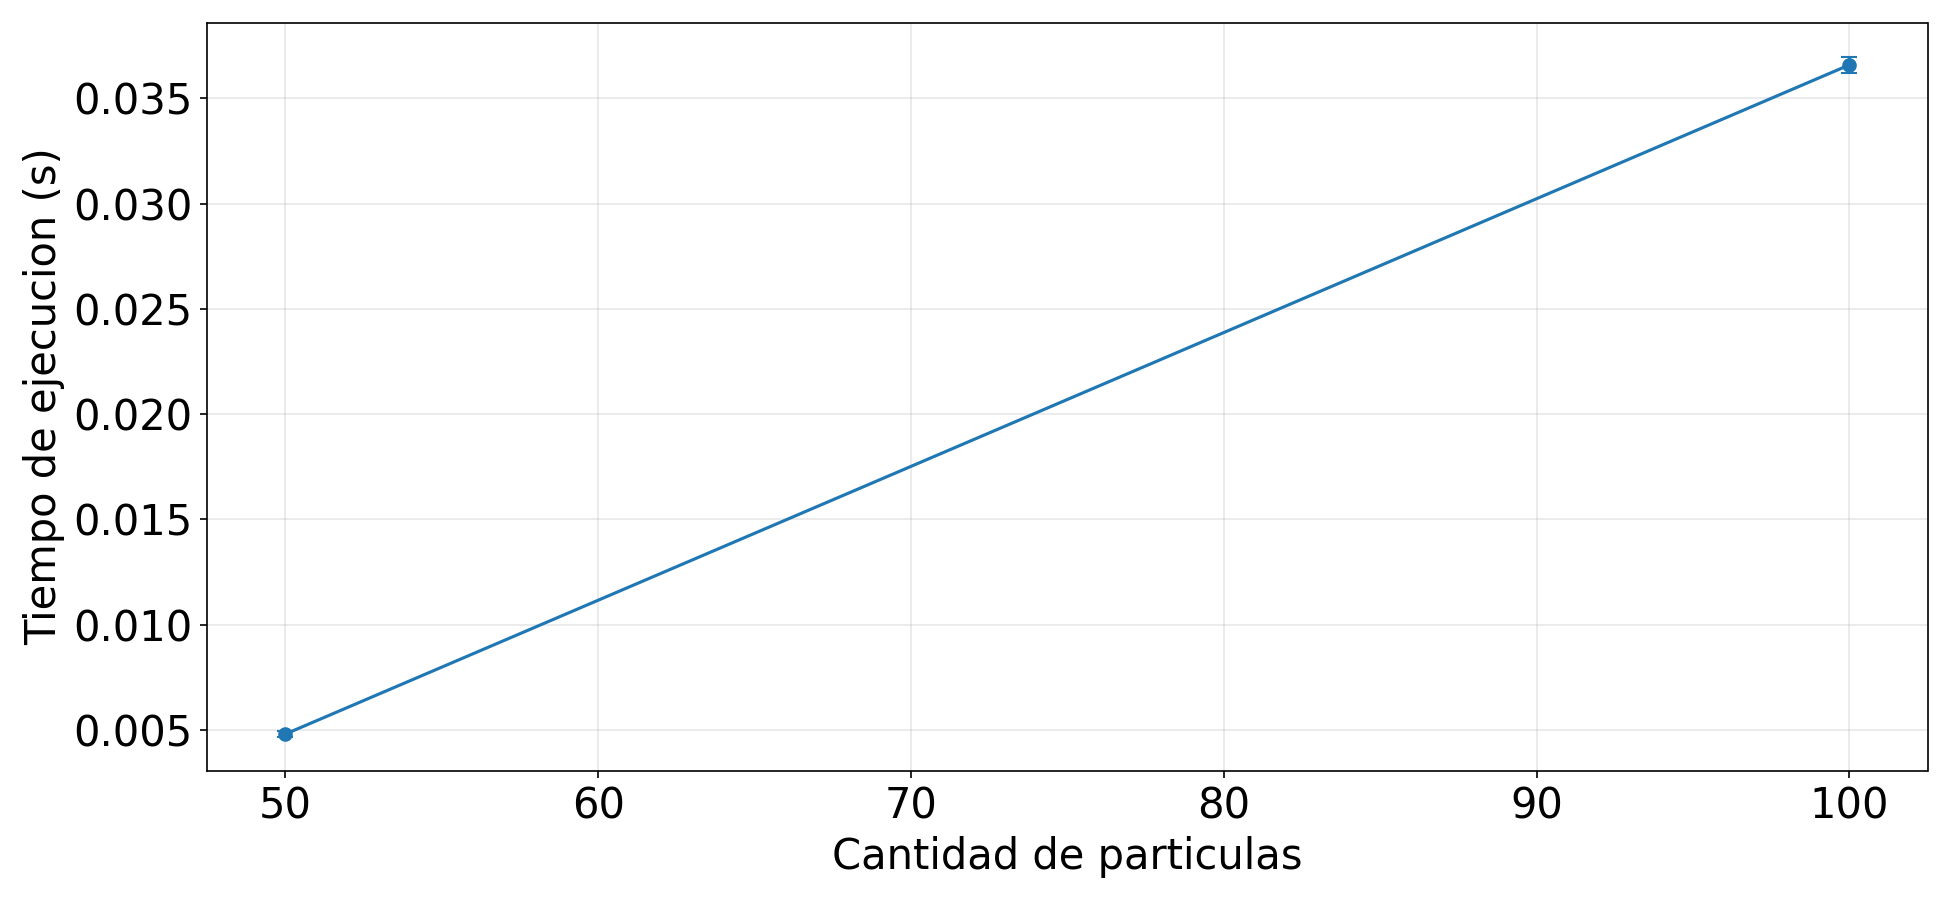
\includegraphics[width=0.75\textwidth]{entrega/1.1/tiempo_ejecucion_vs_n.png}
  \caption{Tiempo de ejecución promedio en función del número de partículas,
    para la mesa sin obstáculos, con $t_f = 30$~s y $v_0 = 1$~m/s. Las barras de
    error corresponden al desvío estándar sobre 10 realizaciones.}
  \label{fig:11-tiempo}
\end{figure}

\subsection{Exploración del espacio de configuraciones}
\label{sec:resultados-configuraciones}

% TODO

\begin{figure}[H]
  \centering
  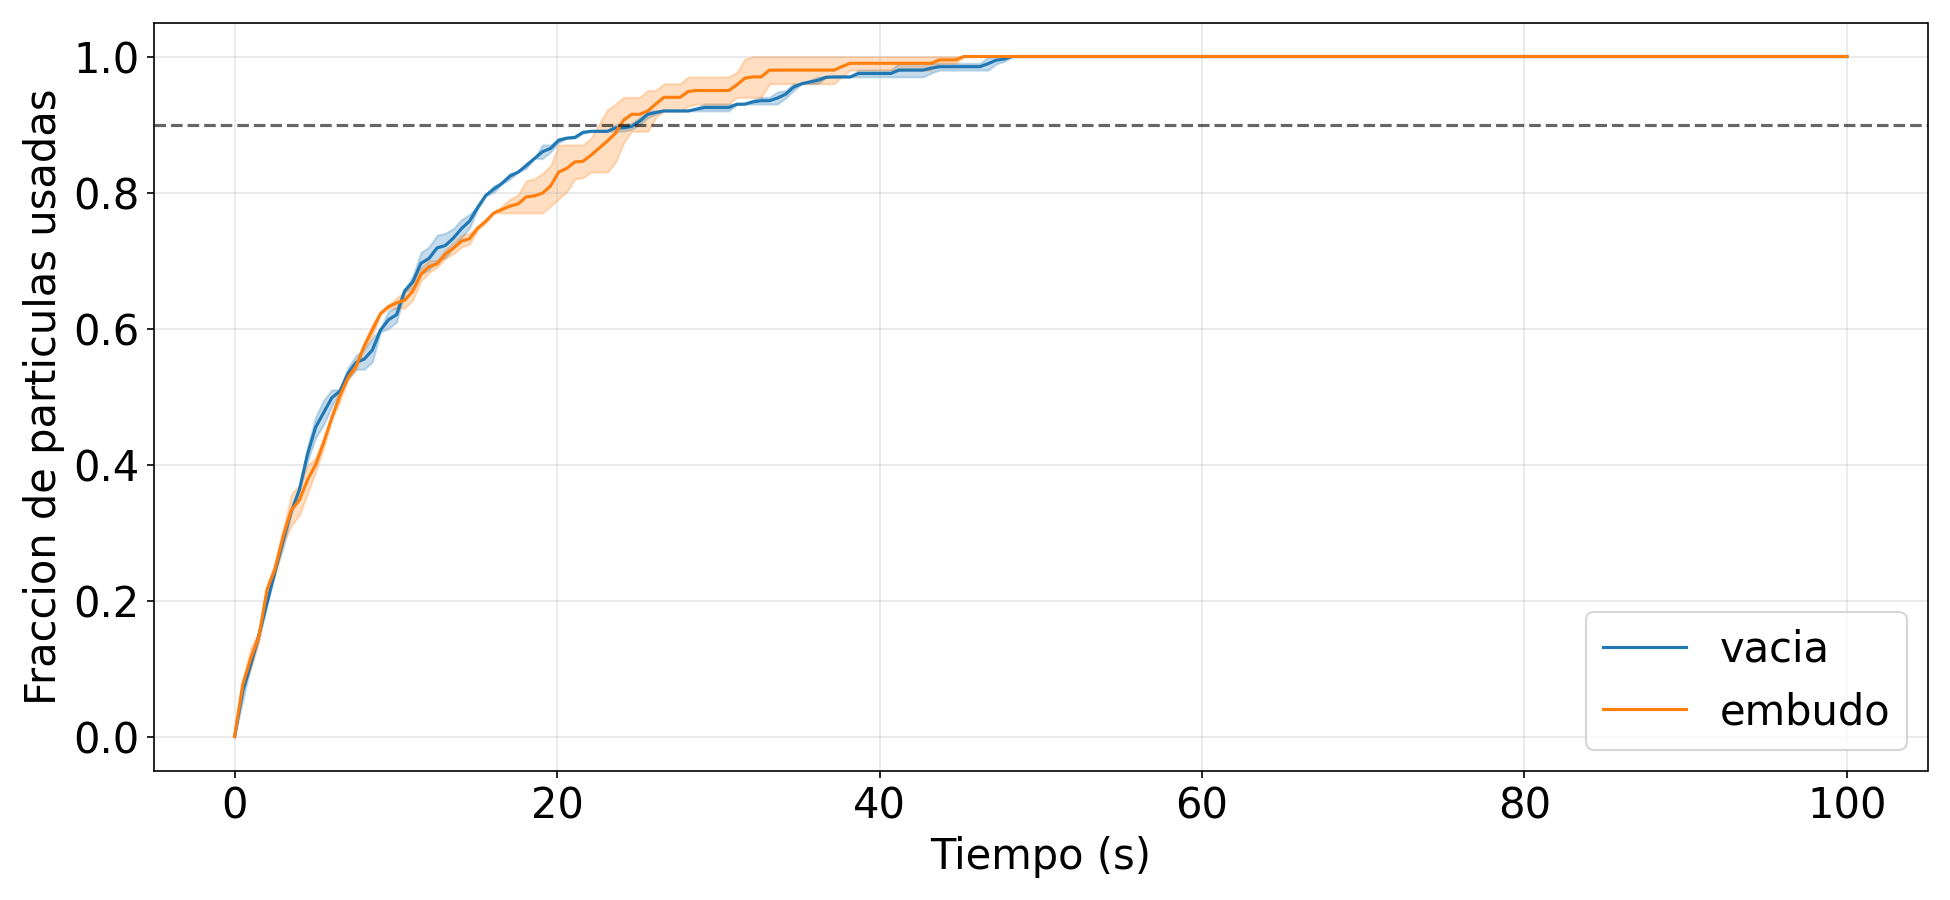
\includegraphics[width=0.8\textwidth]{entrega/1.2/fu_vs_tiempo.png}
  \caption{Fracción de partículas usadas $F_u$ en función del tiempo, para
    $N = 100$ partículas, comparando la mesa vacía contra las configuraciones de
    obstáculos estudiadas. La banda sombreada es el desvío estándar sobre 5
    realizaciones y la línea punteada marca $F_u = 0.9$.}
  \label{fig:12-fu}
\end{figure}

\begin{figure}[H]
  \centering
  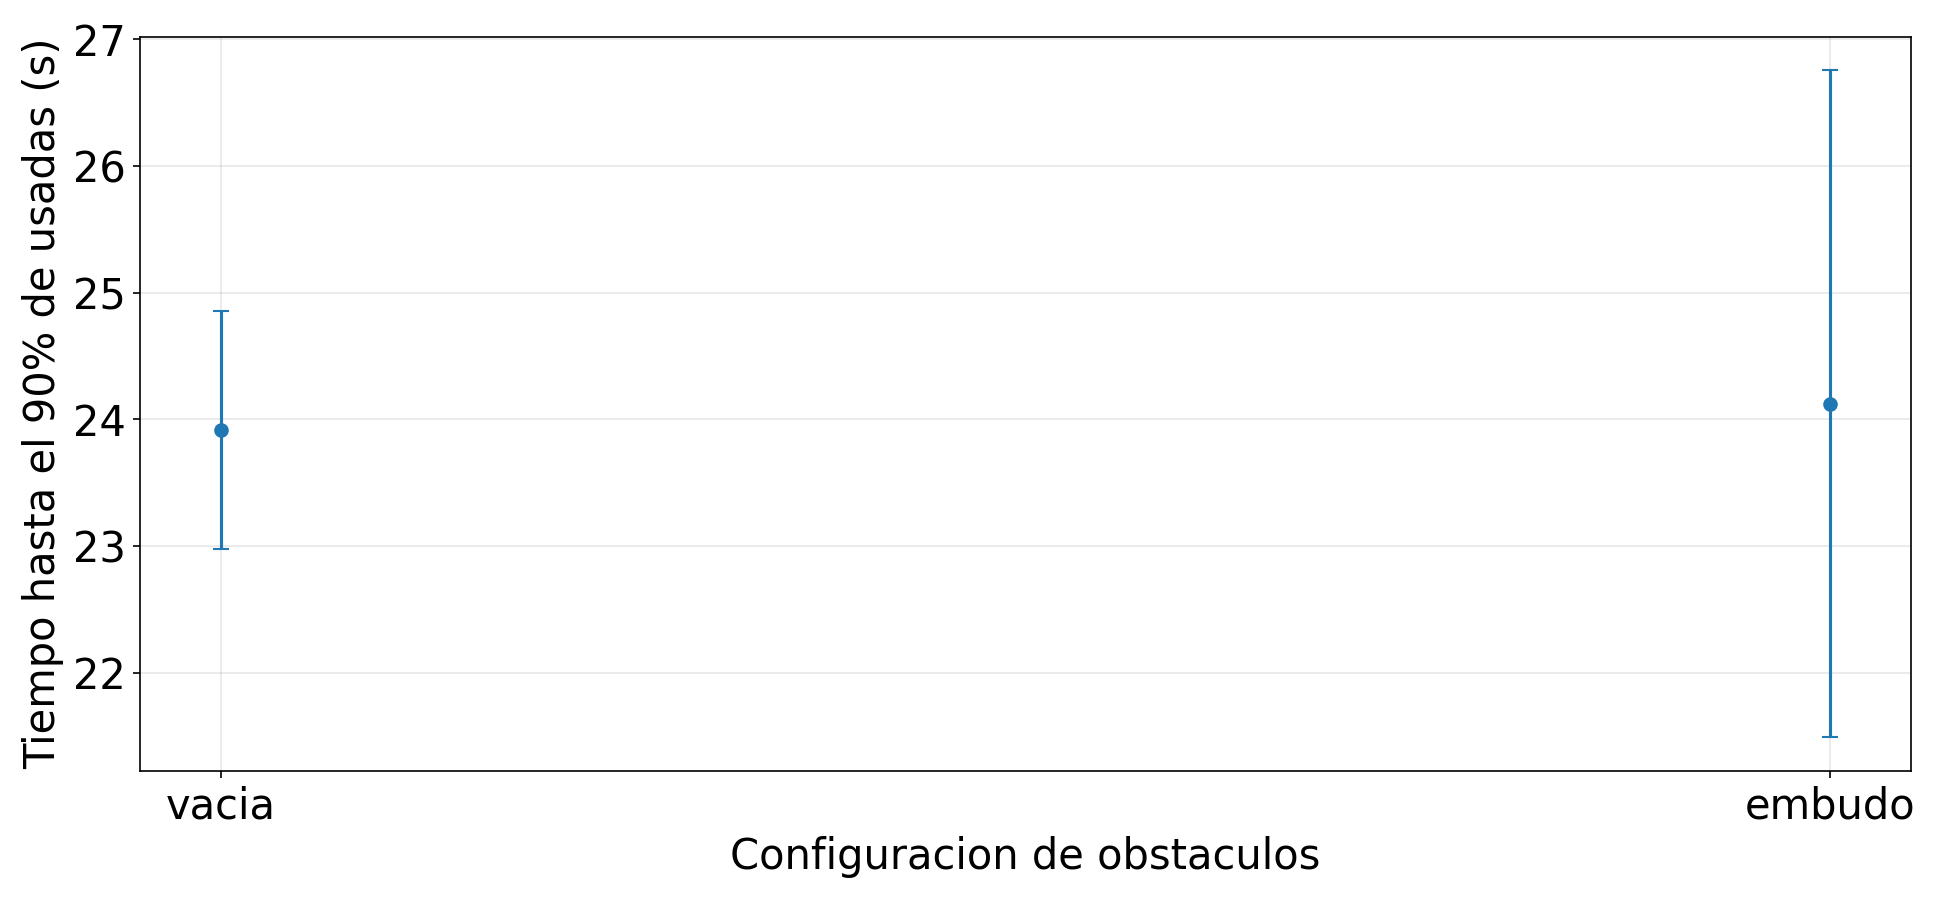
\includegraphics[width=0.75\textwidth]{entrega/1.2/t90_vs_configuracion.png}
  \caption{Tiempo $\tnoventa$ promedio para cada configuración de obstáculos, con
    $N = 100$ partículas y $t_{max} = 100$~s. Las barras de error corresponden al
    desvío estándar sobre 5 realizaciones.}
  \label{fig:12-t90}
\end{figure}

\subsection{Coeficiente de difusión}
\label{sec:resultados-difusion}

% TODO: mencionar el metodo de ajuste de la Teorica 0 y la correlacion entre D
% y <t90>.

\begin{figure}[H]
  \centering
  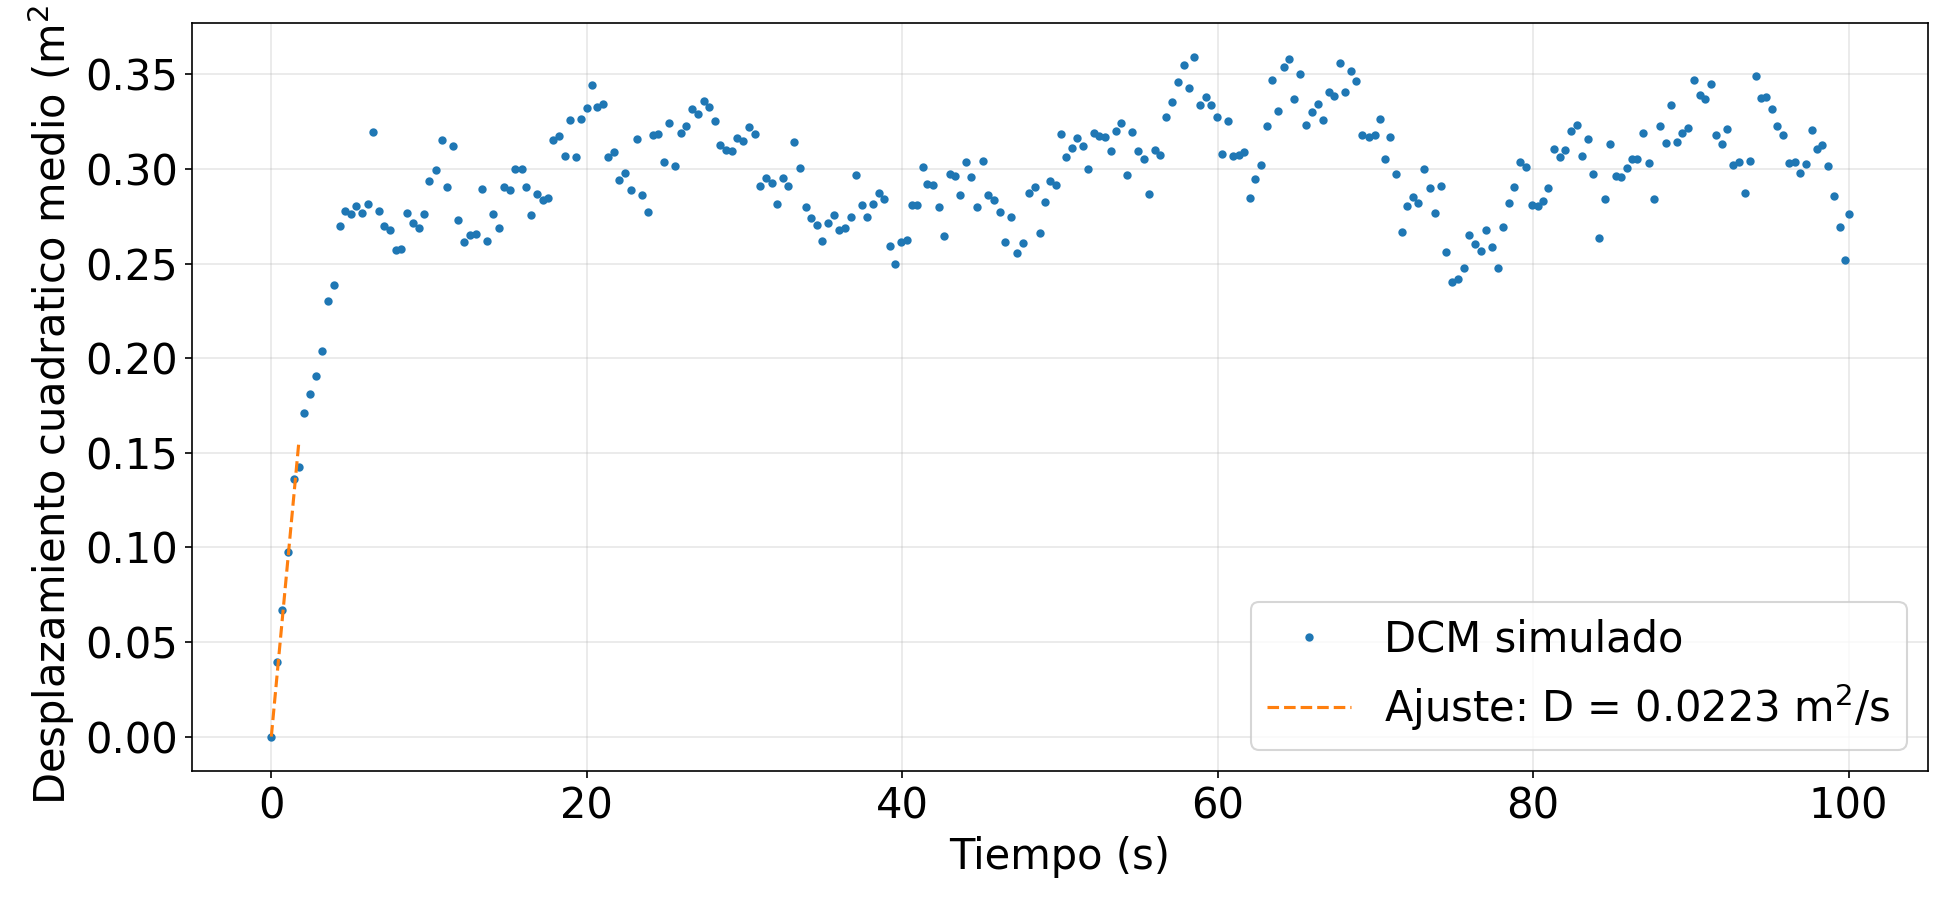
\includegraphics[width=0.8\textwidth]{entrega/1.3/dcm_vacia.png}
  \caption{Desplazamiento cuadrático medio en función del tiempo para una
    realización de la mesa vacía, con $N = 100$ partículas. La línea punteada es
    el ajuste lineal $\mathrm{DCM} = 4Dt$ sobre el tramo inicial.}
  \label{fig:13-dcm-vacia}
\end{figure}

\FloatBarrier
\section{Conclusiones}
\label{sec:conclusiones}

\begin{itemize}
  \item % TODO
  \item % TODO
  \item % TODO
\end{itemize}

\FloatBarrier
\begin{thebibliography}{9}

\bibitem{alder1959}
B. J. Alder, T. E. Wainwright,
``Studies in Molecular Dynamics. I. General Method,''
\emph{The Journal of Chemical Physics}, vol.\ 31, no.\ 2, pp.\ 459--466 (1959).

\end{thebibliography}

\end{document}
